\documentclass[10pt]{beamer}

\usetheme[progressbar=frametitle]{metropolis}
\usepackage{appendixnumberbeamer}
\definecolor{maincolor}{RGB}{35, 55, 58}
\usepackage{booktabs}
\usepackage[scale=2]{ccicons}
\usepackage{tcolorbox}
\tcbuselibrary{theorems}
\usepackage{pgfplots}
\usepgfplotslibrary{dateplot}
\usepackage{xspace}
\usepackage{tikz-cd}
\setbeamercovered{transparent}
\newcommand{\themename}{\textbf{\textsc{metropolis}}\xspace}
\usepackage{graphicx}
\usepackage{subcaption}
\graphicspath{ {./images/} }




% {{{
\def\sh{\mathcal}                   % sheaf font
\def\bb{\mathbb}                    % bold font
\def\cat{\mathtt}                   % category font
\def\leq{\leqslant}                 % <=
\def\geq{\geqslant}                 % >=
\def\setmin{-}                      % set minus
\def\rad{\mathfrak{r}}              % radical
\def\nilrad{\mathfrak{N}}           % nilradical
\def\emp{\varnothing}               % empty set
\def\vphi{\phi}                     % for switching \phi and \varphi, change if needed
\def\HH{\mathrm{H}}                 % cohomology H
\def\CHH{\check{\HH}}               % Čech cohomology H
\def\RR{\mathrm{R}}                 % right derived R
\def\LL{\mathrm{L}}                 % left derived L
\def\dual#1{{#1}^\v}              % dual
\def\v{\smash{\scalebox{.8}[1.4]{\rotatebox{90}{\guilsinglleft}}}}
\def\kres{k}                        % residue field k
\def\C{\cat{C}}                     % category C
\def\op{^\cat{op}}                  % opposite category
\def\Set{\cat{Set}}                 % category of sets
\def\CHom{\cat{Hom}}                % functor category
\def\supertilde{{\,\widetilde{\,}\,}}   % use \supertilde instead of ^\sim
\def\GL{\bb{GL}}
\def\Q{\bb{Q}}
\def\Z{\bb{Z}}
\def\R{\bb{R}}
\def\C{\bb{C}}
\def\O{\sh{O}}
\def\G{\bb{G}}
\def\P{\bb{P}}
\def\bbGamma{\boldsymbol\Gamma}
\def\red{\mathrm{red}}
\def\rg{\operatorname{rg}}
\def\gr{\operatorname{gr}}
\def\Gr{\operatorname{Gr}}
\def\Sym{\operatorname{Sym}}
\def\Hom{\operatorname{Hom}}
\def\Proj{\operatorname{Proj}}
\def\Tor{\operatorname{Tor}}
\def\Ext{\operatorname{Ext}}
\def\Supp{\operatorname{Supp}}
\def\Ker{\operatorname{Ker}}
\def\Im{\operatorname{Im}}
\def\Coker{\operatorname{Coker}}
\def\Spec{\operatorname{Spec}}
\def\Spf{\operatorname{Spf}}
\def\grad{\operatorname{grad}}
\def\dimc{\operatorname{dimc}}
\def\codim{\operatorname{codim}}
\def\id{\operatorname{id}}
\def\Der{\operatorname{Der}}
\def\Diff{\operatorname{Diff}}
\def\Hyp{\operatorname{Hyp}}
\def\Tr{\operatorname{Tr}}
% }}}

\newtcbtheorem{colordef}{Definition} {theorem style = plain, colback=maincolor!30!white, coltitle=black, colframe=black, fonttitle = \upshape\bfseries, fontupper=\itshape}{th}

\newtcbtheorem[no counter]{colorthm}{Theorem} {theorem style = plain, colback=maincolor!30!white, coltitle=black, colframe=white, fonttitle = \upshape\bfseries, fontupper=\itshape}{th}

\newtcbtheorem[no counter]{colorconj}{Conjecture} {theorem style = plain, colback=maincolor!30!white, coltitle=black, colframe=white, fonttitle = \upshape\bfseries, fontupper=\itshape}{conj}

\newtcbtheorem{constructionbox}{Construction} {theorem style = plain, colback=maincolor!30!white, coltitle=black, colframe=black, fonttitle = \upshape\bfseries, fontupper=\upshape}{th}

%\usepackage{floatrow}

\title{Derived categories of coherent sheaves}
% \date{\today}
\date{}
\author{Bogdan Simeonov}
% \titlegraphic{\hfill\includegraphics[height=1.5cm]{logo.pdf}}

\begin{document}

\maketitle
%Computer Project?

\begin{frame}{Overview}
    \begin{itemize}
        \pause
        \item 
    \end{itemize}
 
\end{frame}

\begin{frame}{Rationality of cubic fourfolds}
    We know classically that cubic curves are not rational (they are elliptic curves). However, cubic surfaces are always rational! Clemens and Griffiths showed in 1972 that cubic threefolds are, in contrast, never rational.

    What about cubic fourfolds?
\end{frame}

\begin{frame}[fragile]{Hodge theory of the cubic fourfold}
    Let $X\subset \P^5$ be the zero locus of a degree $3$ polynomial. We can compare its Hodge diamond to that of a K3 surface: 

                            %\captionsetup{justification=centering}
                        %   \begin{center}
                                %\hfill
                                
                        %       \begin{minipage}[t]{0.4\textwidth}
                        %       \centering
                        %           \begin{figure}[H]
                        %           \begin{tikzcd}[ampersand replacement=\&, row sep=0.10em, column sep=0.10em]
                        %               \\
                        %               \\
                        %               \\
                        %               \\
                        %               \\
                        %               \\
                        %               \\
                        %               \\
                        %               \\
                        %               \\
                        %               \\
                        %               \\
                        %               \\
                        %              \\
                        %              \\
                        %               \\
                        %               \\
                        %               \\
                        %               \\
                        %               \\
                        %               \\
                        %               \\
                        %               \\
                        %               \\
                        %               \\
                        %               \\
                        %               \\
                        %               \\
                        %               \\
                        %               \\
                        %               \&   \& 1  \&   \&   \\
                        %               \& 0 \&    \& 0 \&   \\
                        %           1 \&   \& 20 \&   \& 1 \\
                        %               \& 0 \&    \& 0 \&   \\
                        %               \&   \& 1  \&   \& 
                        %           \end{tikzcd}
                        %
                        %            \caption*{Hodge diamond of K3 surface} \label{fig: MonFun2}
                        %            \end{figure}
                        %        \end{minipage}
                        %        %\captionsetup{justification=centering}
                        %        \begin{minipage}[t]{0.4\textwidth}
                        %        \centering
                        %            \begin{figure}[H]
                        %            \begin{tikzcd}[ampersand replacement=\&, row sep=0.10em, column sep=0.10em]
                        %                \&   \&   \&   \& 1  \&   \&   \&   \&   \\
                        %                \&   \&   \& 0 \&    \& 0 \&   \&   \&   \\
                        %                \&   \& 0 \&   \& 1  \&   \& 0 \&   \&   \\
                        %                \& 0 \&   \& 0 \&    \& 0 \&   \& 0 \&   \\
                        %            0 \&   \& 1 \&   \& 21 \&   \& 1 \&   \& 0 \\
                        %                \& 0 \&   \& 0 \&    \& 0 \&   \& 0 \&   \\
                        %               \&   \& 0 \&   \& 1  \&   \& 0 \&   \&   \\
                        %                \&   \&   \& 0 \&    \& 0 \&   \&   \&   \\
                        %                \&   \&   \&   \& 1  \&   \&   \&   \& 
                        %            \end{tikzcd}
                        %            \centering\caption*{\,\,\,\,\,\,\,\,Hodge diamond of X} \label{fig: MonFun3}
                        %            \end{figure}
                        %        \end{minipage}
                            %\hfill
                            %\null
                        %    \end{center}
\begin{figure}
    \centering
    \begin{minipage}{0.45\textwidth}
        \centering
        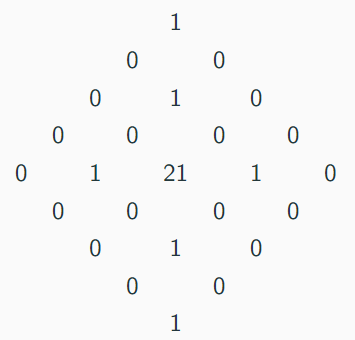
\includegraphics[width=0.9\textwidth]{CubicFourfoldHodgeDiamond.png} % first figure itself
        \caption*{Cubic fourfold}
    \end{minipage}\hfill
    \begin{minipage}{0.45\textwidth}
        \centering
        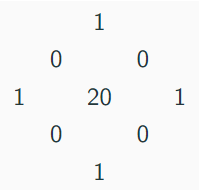
\includegraphics[width=0.4\textwidth]{K3diamond} % second figure itself
        \caption*{K3 surface}
    \end{minipage}
\end{figure}

\end{frame}

\begin{frame}{The moduli space of cubic fourfolds}
    Both K3 surfaces and cubic threefolds have a Global Torelli theorem, meaning that a cubic fourfold is specified by the line $H^{3,1}\subset H^4$, the condition $H^{3,1}\perp h^2$ and furthermore $\eta\cup \eta =0, \eta \cup \overline{\eta}>0$ and so the period map lands in an open subset of a quadric in $\P^{21}$. Voisin proved that this is an open immersion.
\end{frame}

\begin{frame}{Cubic fourfolds and K3 surfaces}
    If we take the primitive cohomology of the cubic fourfold, we get something that looks exactly like a K3 surface! However, the two have different signatures.
    To be able to compare them, we have to pass to a codimension one subspace. For the K3, we can always take the primitive cohomology. \pause For \emph{special cubic fourfolds} we can find a class $T\in H^{2,2}(X,\mathbb{Z})$ and move to its orthogonal complement.\pause

    \begin{colorthm}{Hasset}{}
        The cubics containing an integral class $T$ as above form a family of irreducible divisors $\mathcal{C}_d$, nonempty iff $d>6, d=0,2 \,( \mathrm{mod}\, 6)$. Moreover, the cubics in $\mathcal{C}_d$ have an associated K3 surface i.e. $\exists S$ such that $$H^2_{prim}(S)\simeq \langle h^2, T\rangle ^\perp$$
        precisely when $d$ is not divisible by four, nine, or any odd prime $p =-1(\,\mathrm{ mod }\, 3)$
    \end{colorthm}
\end{frame}

\begin{frame}{Back to the rationality problem for cubic fourfolds}

    Implicit in Hasset's results is the conjecture that the special cubic fourfolds are rational. Intuitively, one has to blow up a surface in order to be birational to $\P^4$. Hence, we expect the rational cubic fourfolds to form a countable union of divisors, which is neither open nor closed, in stark contrast to the lower dimensional cases!
    
\end{frame}

\begin{frame}{The derived perspective}
    Kuznetsov presented a different viewpoint on the cubic fourfold using derived categories. The three line bundles $\mathcal{O}_X, \mathcal{O}_X(1), \mathcal{O}_X(2)$ form an exceptional collection and he defined the component $$\mathcal{A}_X=\langle \mathcal{O}_X, \mathcal{O}_X(1), \mathcal{O}_X(2)\rangle ^\perp\subset \mathcal{D}(X)$$\pause

    The HKR theorem guarantees that the Hochschild homology of $\mathcal{A}_X$ is the same as that of a K3 surface. \pause Kuznetsov showed that $\mathcal{A}_X$ is a \emph{Calabi Yau 2} category and we can think of $\mathcal{A}_X$ as a noncommutative K3 surface.\pause

    \begin{colorconj}{Kuznetsov}{}
        $X$ is rational if and only if there is a K3 surface $S$ such that $$\mathcal{D}(S)\simeq \mathcal{A}_X$$
    \end{colorconj}
    
\end{frame}

\begin{frame}{(Non)-example: cubics containing a plane}
    
\end{frame}










    

\end{document}
